\section{LSTM}
\label{section:lstm}
Το Μοντέλο Long Short-Term Memory (LSTM) αποτελεί ένα είδος αναδρομικών νευρωνικών δικτύων, σχεδιασμένο για την αντιμετώπιση προβλημάτων που συνδέονται με την ανάλυση και την πρόβλεψη χρονοσειρών. Το LSTM model διαθέτει μια αναδρομική δομή που του επιτρέπει να διατηρεί και να χρησιμοποιεί πληροφορίες από προηγούμενες χρονικές στιγμές. Αυτό είναι κρίσιμο για την αντιμετώπιση μακροπρόθεσμων εξαρτήσεων στα δεδομένα. 

Το LSTM έχει μια αναδρομική δομή, που σημαίνει ότι μπορεί να αποθηκεύει πληροφορίες από προηγούμενες χρονικές στιγμές. Κάθε μονάδα LSTM διαθέτει τρεις βασικές πύλες για τον έλεγχο της ροής των πληροφοριών:

\begin{enumerate}
    \item Πύλη Εισόδου (Input Gate): Η πύλη εισόδου καθορίζει ποιες νέες πληροφορίες θα αποθηκευτούν στην κυτταρική μνήμη. Είναι υπεύθυνη για την επιλογή του ποσοστού πληροφοριών που θα εισέλθουν στον κυτταρικό χώρο. Η διαδικασία αυτή συμβάλλει στη δημιουργία νέων μνημονικών αποτυπωμάτων με βάση τα νέα δεδομένα που εισέρχονται.
    \item Πύλη Εξόδου (Output Gate): Η πύλη λήθης είναι υπεύθυνη για την απόφαση, του ποιες πληροφορίες θα "ξεχαστούν" ή θα διαγραφούν από την κυτταρική μνήμη. Αυτή η λειτουργία βοηθά στο να αποφεύγεται η συσσώρευση ανεπιθύμητων πληροφοριών που δεν είναι πλέον σημαντικές για την πρόβλεψη.
    \item Πύλη Λήθης (Forget Gate): Η πύλη εξόδου αποφασίζει ποια πληροφορία από την κυτταρική μνήμη θα εξαχθεί ως τελική έξοδος της μονάδας LSTM. Ελέγχει το ποσοστό της μνημονικής πληροφορίας που θα συνεισφέρει στο τελικό αποτέλεσμα. Αυτή η πύλη καθορίζει την τελική έξοδο της LSTM μονάδας.
\end{enumerate}

\begin{figure}[!ht]
	\centering
	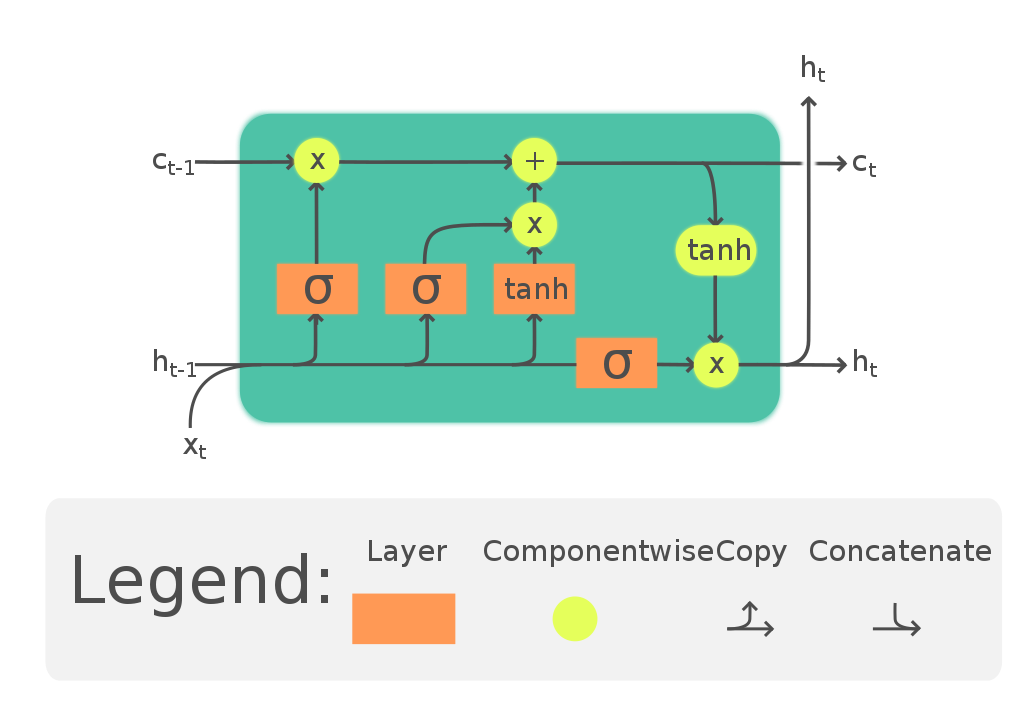
\includegraphics[width=0.7\textwidth]{./images/chapter2/LSTM_Cell.png}
	\caption[Σχηματική απεικόνιση Long-Short Term Memory cell]{Σχηματική απεικόνιση Long-Short Term Memory cell} \cite{pictlstm}
	\label{fig:LSTM_Cell}
\end{figure}

Η διαχείριση αυτών των πυλών επιτρέπει στο LSTM να διατηρεί και να χρησιμοποιεί μακροπρόθεσμες εξαρτήσεις στα δεδομένα, καθιστώντας το ιδιαίτερα αποτελεσματικό στη χρονοσειριακή ανάλυση και πρόβλεψη.

Κάθε κύτταρο του LSTM περιέχει μνήμη. Η μνήμη κυττάρου είναι υπεύθυνη για την αποθήκευση και τη διατήρηση των πληροφοριών. Αυτή η δομή επιτρέπει στο μοντέλο να αντιλαμβάνεται και να ανταποκρίνεται σε μακροπρόθεσμες συναρτήσεις στα δεδομένα. Με τον τρόπο αυτό, το LSTM model εκπαιδεύεται να αναγνωρίζει προτεραιότητες, τάσεις και μοτίβα στα δεδομένα χρονοσειρών, παρέχοντας ένα πολύ ισχυρό εργαλείο για την πρόβλεψη μελλοντικών τιμών και την ανίχνευση ανωμαλιών.

Η εφαρμογή του LSTM model στην παρακολούθηση συστημάτων προσφέρει ποικίλα οφέλη που απορρέουν από την εξελιγμένη του λειτουργία. Η αρχιτεκτονική του LSTM model επιτρέπει την ακριβή πρόβλεψη των επιπέδων φόρτου του συστήματος. Αυτό είναι ιδιαίτερα σημαντικό για την πρόληψη υπερφόρτωσης και την αποτελεσματική διαχείριση των πόρων. Ένα από τα ισχυρά σημεία του LSTM model είναι η ικανότητά του να προσαρμόζεται αυτόματα σε νέες συνθήκες, διατηρώντας την απόδοσή του σε ποικίλες μεταβαλλόμενες συνθήκες.
Χάρη στην αναδρομική δομή, τις πύλες και τη διαχείριση μνήμης κάθε cell, το LSTM model αποτελεί ιδανική επιλογή για παρακολούθηση χρονοσειρών. Με τον τρόπο αυτό, το LSTM model χρησιμοποιείται σε πρόβλεψη σεισμών, την παρακολούθηση κίνησης οχημάτων εκτός δρόμου, την πρόβλεψη κίνησης τροφοδοσίας σε συστήματα ηλεκτρικής ενέργειας, στην πρόβλεψη κυκλοφοριακής συμφόρησης αλλά και στην πρόβλεψη κατανάλωσης ενέργειας σε κτίρια.
